\section{Project description}
\label{chapter1}

The Project description section provides a brief overview of the project, covering the basic idea with simple sketches for visualization.

\subsection{Problem description}

%FIXME: De-uglify diagram (Lorenzo)

The aim of the project is to develop a simplified adaptive cruise control (ACC) system based on two Raspberry Pi 4 devices communicating with each other via Bluetooth. Node 1 is responsible for collecting environmental data using ultrasonic sensors, while Node 2 controls the vehicle speed and interacts with the user via a touch display.

\begin{figure}[h]
	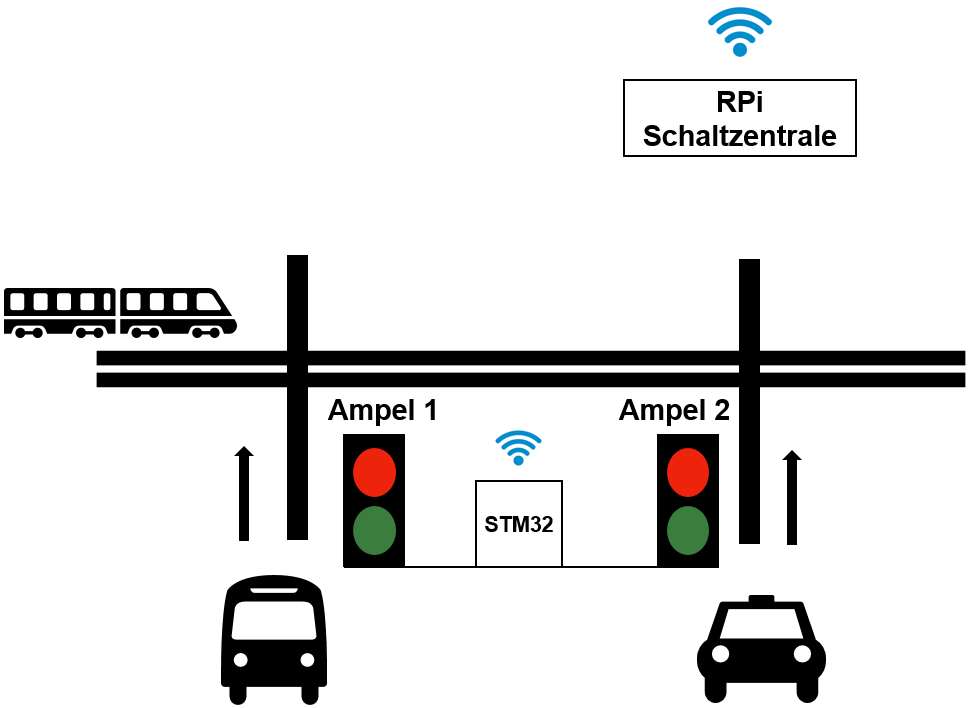
\includegraphics[height=100mm]{images/system}
	\centering
	\caption{system description}
	\label{fig:system}
\end{figure}

\paragraph{}
%The adaptive cruise control (acc) system consists of two nodes, node1, and node2. The nodes are connected by a (FIXME: encrypted/authenticated/both) bluetooth link.

\paragraph{}
Node 1 is equipped with two HC-SR04 ultrasonic sensors that detect cars in front of a virtual vehicle. It performs measurements with both sensors, checks their results for consistency and plausibility, and then transmits the validated values to Node 2. Instead of distance data, the sensor message may also contain error status information which has a different value range than ordinary distance data. The error assumption is that at most one of the two sensors can fail within a defined period of time.

\paragraph{}
Node 2 takes over the function of the steering control unit (ECU) of the virtual vehicle. A control panel on the display can be used to manually increase or decrease the speed of the vehicle, while an additional switch turns the adaptive cruise control (ACC) system on or off. The display shows the current speed and distance values, and the operating status of the ACC (active/inactive/error). Depending on the ACC state, a virtual status display either glows green (active/inactive) or red (error). The requirements for status display, speed and distance displays, and user input can be conveniently implemented using a touchscreen display, for example, with a corresponding \href{https://www.berrybase.at/raspberry-pi-touch-display-2-7-portrait} {Raspberry Pi-compatible device}. 

\paragraph{}
\textbf{Hardware used:}
\begin{itemize}
    \item 2 × Raspberry Pi 4B
    \item 2 × HC-SR04 Ultrasonic Sensor
    \item 1 × Raspberry Pi Touch Display 2, 7" Portrait
\end{itemize}
